\section{Further Research Trends}

electrical muscle stimulation ?

electrical nerve stimulation ?

\subsection{Improvements For VR Games}
\subsubsection{General Input}

\begin{itemize}
	\item controller
	\item sound
	\item photo electric effects
\end{itemize}

\subsubsection{Movement}
How Players can move better in VR (e.g. without becoming cybersik)

\begin{itemize}
	\item point and teleport
	\item walk (with moving floor tiles?)
	\item player does not move, but rather the environment around him (car, train, airplane)
	\item stationary weapons/tasks
\end{itemize}

\subsubsection{Feel}
How Users can feel items from the virtual environment in the real world (shape changing UIs)

\subsubsection{Taste}
How other senses can be included into VR

Ranasinghe, Nimesha and Do, Ellen Yi-Luen~\cite{Ranasinghe:2016:VSS:2984751.2985729} have developed a way to address the tastebuds using electrical stimulation

\todo[inline]{JF: Das hier ist vielleicht noch interessant zu dem was in Zukunft gemacht wird:
\url{https://www.youtube.com/watch?v=Mv_eIRv1Vk4}}

\subsubsection{Hearing}
Is there sufficient research in hearing in VR? (not every user has some 5.1 sound system at home)

\subsection{Health Aspects}

\begin{itemize}
	\item cybersickness
	\item psychological profits (people with psycological(?) illness can be treated)
	\item psychological disadvantages (people can confuse VR with reality)
\end{itemize}

\subsubsection{Physical Health}
How VR can help with physical health, although stuff like the WII fit better for this purpose

Health care training for professional workers in health-care

\subsubsection{Mental Health}
Could VR games help treat people with mental problems (VR is more immense than normal games)

Can Training in a Real-Time Strategy Videogame Attenuate Cognitive Decline in Older Adults?

Action video game modifies visual selective attention

\subsection{Physical Objects}

Using some similar technology to the iDummy\footnote{"IDummy" IDummy Product Website, 2015, accessed November 05., 2016, \url{http://www.idummy.com/}} one can create various objects of different size and shape. A user wearing a VR Headset can see a specific object and feel it as if it was the real thing. Using the technology developers can extend the realm of VR to one more dimension. Together with the technology~\cite{Azmandian:2016:HRD:2858036.2858226}

Using something similar to the modular tiles creating levels in portal (a 100x100 cm tile is attached to a robotic arm)

\begin{figure}
	\centering
	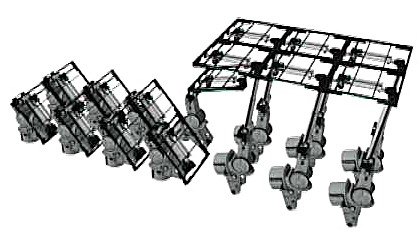
\includegraphics[width=0.9\columnwidth]{./figures/portallabrattest}
	\caption[Portal 2 : Lab Rat Panel Test]{Screenshot from the promotional video 'Portal 2 : Lab Rat Panel Test' (\ccbyncsa) of the game \textit{Portal 2 \textregistered\textcopyright} showing the general setup of floor panels mounted to robotic arms. This method enables developers to modify the structure of the floor at runtime.\footnotemark}~\label{fig:portallabrattest}
\end{figure}
\footnotetext{\textcopyright "Valve Software", Portal 2, [Online; accessed November 05., 2016],[Digitally revised] \url{https://www.youtube.com/watch?v=S7vFxs0ycn0}}

I can think of an application where the tiles are intelligently configured to 'disapear' (into the ground) behind the player and appear in front of him (out of the ground again) kind of like a hamster wheel, macking the playable area seem infinitely large to the player. Kind of like in Portal~\cite{game:portal} video game.

Approaches like the one taken by Hiroo Iwata, Hiroaki Yano, Hiroyuki Fukushima in their CirculaFloor~\cite{Iwata:2005:CLI:1078037.1079777} or~\cite{Souman:2010:MVW:1670671.1670675} go are interesting and should be further investigated. 

%\textcolor{gray}{\blindtext[3]}

\subsection{Increasing The Performance Of Devices For VR Gaming}
How can VR leave the living room for good?

\todo[inline]{JF: Wieso sollte es denn aus dem Wohnzimmer raus? Das ist doch gerade für den Anwendungsfall der Zielbereich}

\todo{Warum 90fps?? \url{https://www.reddit.com/r/oculus/comments/3zgva1/why_is_constant_90_fps_so_important_in_vr/}}
%\textcolor{gray}{\blindtext[1]}
